
\chapter{Overall Description} \label{chp:overall-description}

\section{Product Perspective}
	\begin{comment}
		$<$Describe the context and origin of the product being specified in this SRS.  
		For example, state whether this product is a follow-on member of a product 
		family, a replacement for certain existing systems, or a new, self-contained 
		product. If the SRS defines a component of a larger system, relate the 
		requirements of the larger system to the functionality of this software and 
		identify interfaces between the two. A simple diagram that shows the major 
		components of the overall system, subsystem interconnections, and external 
		interfaces can be helpful.$>$
	\end{comment}

	The idea of simulation tool started with the process of acquiring a new supercomputer in order to support research activities by university. The need of a new product was established by replacing the existing system to a newer one. Simulation tool is a new-born, self-contained product which will be used in order to get the best accounting practices. 	
	\begin{wrapfigure}{r}{0.5\textwidth} 
		\centering
		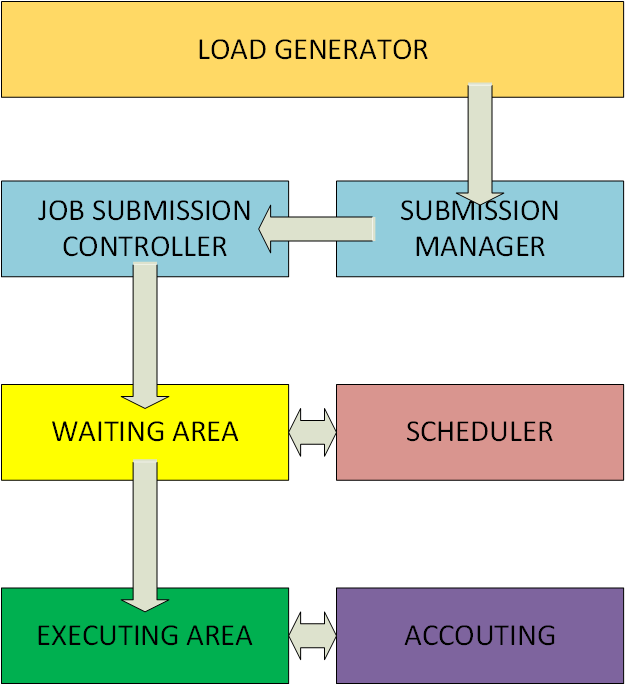
\includegraphics[scale=0.4]{../visio-files/components}
		\caption{Block diagram of simulator.}
		\label{fig:block-diagram-of-simulator}
	\end{wrapfigure}

	Simulator can be divided into two parts which are independent from each other. The first part is a load generator, which simulates a given job and overall requested directed to computation platform. The second part is a processing routine which takes care of incoming/already received and executing tasks. This fragmentation can be divided again in terms of second part which is shown in Figure \ref{fig:block-diagram-of-simulator}. After receiving tasks by \emph{Submission Manger} the task/job is conveyed to \emph{Job Submission Controller}, which search for a best-matching queue (executing area) for a given job. First place where a job is placed is \emph{Waiting Area}, which is managed by a \emph{Scheduler} which is a algorithm that determines an order of a tasks to be moved into \emph{Executing Area}. If task started its execution the \emph{Accouting} module takes care of billing in terms of time and used resources.
		
	Tool is a closed for changes in terms of scheduling and accounting algorithm, although the configurations can vary from one simulation to another. There is only one input interface of communication -- configuration file which is consumed by a program and one output interface -- output of the simulation.
\section{Product Functions}
	\begin{comment}
		$<$Summarize the major functions the product must perform or must let the user 
		perform. Details will be provided in Section 3, so only a high level summary 
		(such as a bullet list) is needed here. Organize the functions to make them 
		understandable to any reader of the SRS. A picture of the major groups of 
		related requirements and how they relate, such as a top level data flow diagram 
		or object class diagram, is often effective.$>$
	\end{comment}
	The main function of a software is to perform simulation for different conditions of accounting practice. In order to simulate behavior of \gls{computing-platform} user should determine following configuration properties: 
	\begin{itemize}
		\item Number of computational nodes, amount of cores, their type and pricing;
		\item Machine operational cost per unit time;
		\item
		{
			Queues properties:
			\begin{itemize}
				\item Cost of core usage per time unit;
				\item Maximum execution time;
				\item Working time range;
				\item Restrictions of allocation of resources.
			\end{itemize}
		}
		\item
		{
			Amount of users and their budget;
		}
		\item Simulation time and/or stop condition.
	\end{itemize}
	
	The outcome of simulation will be presented in a simple report in form of text file. Main flow of the data is shown in Figure \ref{fig:main-flow-of-data}.
	
	\begin{figure}
		\centering
		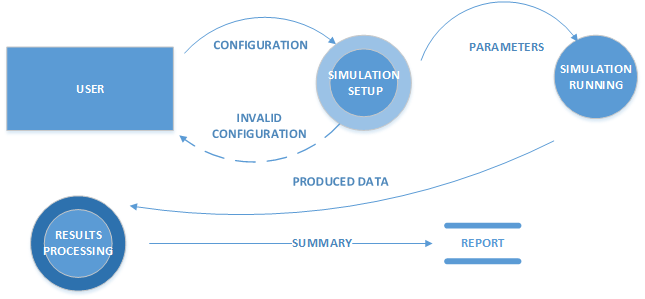
\includegraphics[width=\textwidth]{../visio-files/main-flow-of-data}
		\caption{Main flow of data in simulator.}
		\label{fig:main-flow-of-data}
	\end{figure}
\section{User Classes and Characteristics}
	\begin{comment}
		$<$Identify the various user classes that you anticipate will use this product.  
		User classes may be differentiated based on frequency of use, subset of product 
		functions used, technical expertise, security or privilege levels, educational 
		level, or experience. Describe the pertinent characteristics of each user class.  
		Certain requirements may pertain only to certain user classes. Distinguish the 
		most important user classes for this product from those who are less important 
		to satisfy.$>$
	\end{comment}

\section{Operating Environment}
	\begin{comment}
		$<$Describe the environment in which the software will operate, including the 
		hardware platform, operating system and versions, and any other software 
		components or applications with which it must peacefully coexist.$>$
	\end{comment}

\section{Design and Implementation Constraints}
	\begin{comment}
		$<$Describe any items or issues that will limit the options available to the 
		developers. These might include: corporate or regulatory policies; hardware 
		limitations (timing requirements, memory requirements); interfaces to other 
		applications; specific technologies, tools, and databases to be used; parallel 
		operations; language requirements; communications protocols; security 
		considerations; design conventions or programming standards (for example, if the 
		customer’s organization will be responsible for maintaining the delivered 
		software).$>$
	\end{comment}

\section{User Documentation}
	\begin{comment}
		$<$List the user documentation components (such as user manuals, on-line help, 
		and tutorials) that will be delivered along with the software. Identify any 
		known user documentation delivery formats or standards.$>$
	\end{comment}

\section{Assumptions and Dependencies}
	\begin{comment}
		$<$List any assumed factors (as opposed to known facts) that could affect the 
		requirements stated in the SRS. These could include third-party or commercial 
		components that you plan to use, issues around the development or operating 
		environment, or constraints. The project could be affected if these assumptions 
		are incorrect, are not shared, or change. Also identify any dependencies the 
		project has on external factors, such as software components that you intend to 
		reuse from another project, unless they are already documented elsewhere (for 
		example, in the vision and scope document or the project plan).$>$
	\end{comment}

